\documentclass[english,11pt, reqno, oneside]{amsart}
\usepackage{amsmath}
\usepackage{amssymb}
\usepackage[usenames,dvipsnames]{xcolor}
\usepackage[colorlinks=true,linkcolor=blue!95!black, citecolor = green!55!black,bookmarksdepth=3]{hyperref}
\usepackage{tikz}
\usetikzlibrary{calc}
\usetikzlibrary{math}
\usetikzlibrary{decorations.markings, decorations.pathreplacing,shapes.misc}

\begin{document}

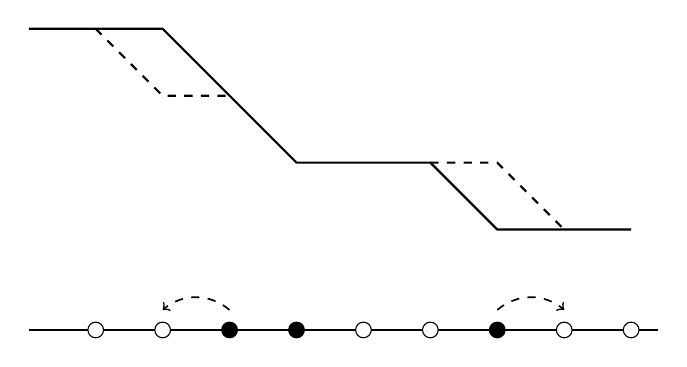
\begin{tikzpicture}[scale=0.85]
\draw[thick] (0,0) -- ++(2,0) -- ++(2,-2) -- ++(1,0) -- ++ (1,0) -- ++(1,-1) -- ++(2,0);

\draw[thick] (0,-4.5) -- ++(9.4,0);

\foreach \thecolor [count=\x] in {white, white, black, black, white, white, black, white, white}
\node[circle, fill=\thecolor, inner sep = 2pt, draw=black] at (\x,-4.5) {};


\draw[->, dashed, semithick] (7, -4.2) to[out=40, in=140] (8,-4.2);

\draw[->, dashed, semithick] (3, -4.2) to[out=140, in=40] (2,-4.2);

\draw[thick, dashed] (1,0) -- ++(1,-1) -- ++(1,0);
\draw[thick, dashed] (6,-2) -- ++(1,0) -- ++(1,-1);
\end{tikzpicture}

\end{document}